\chapter{Design}

% Containing a comprehensive description of the design chosen, how it addresses the problem, and why it is designed the way it is.
Although carrying out a significant amount of up-front design has been avoided, there are some high-level design decisions that have been researched and made in advance, to underpin the development process. These key design decisions surrounding system architecture, the message threading model, and user interface design are outlined below.

\section{High-Level System Architecture}\label{sec:high-level-architecture}

High-level architectural design decisions for this project have been heavily influenced by the requirement that the entire system should be federated, not relying on services from any individual provider. A number of possible architectural models were proposed as a result of research and these possibilities are outlined below.

\begin{enumerate}
  \item \label{itm:web-cloud} A web based system, hosted on a cloud service provider such as Amazon Web Services (AWS), Google Cloud Platform (GCP) or Microsoft Azure.
  \item \label{itm:on-demand-cloud} A locally installed application which spins up a compute instance on a cloud service provider on demand for each user for handling computationally expensive work.
  \item \label{itm:local-service} A locally running web-based user interface which communicates via standard web protocols such as HTTP with a separate locally running service process.
  \item \label{itm:electron} An application which encapsulates the frontend user interface and backend service into a single executable that can be run locally.
\end{enumerate}

Each of the models listed above present their own advantages and disadvantages. Although Model \ref{itm:web-cloud}, an entirely web-based system, would mean that the software is accessible from anywhere, by any device with a web browser, which would improve the user experience, it also means that users have no choice but to trust the backend of this software, running in the cloud, with their data, which means that the federated aspect of the system is lost and privacy concerns are not resolved.

In Model \ref{itm:on-demand-cloud}, users would have more control over their data in the cloud, as they are responsible for managing the cloud compute instance, however implementing this model would mean that users are required to have in-depth knowledge of AWS or similar, which detracts from the usability of the system, violating the non-functional requirement that the application should be easy to set up and use.

The solution proposed in Model \ref{itm:local-service} does not rely on any remotely hosted software, and so maintains the integrity of the federated system, ensuring that the user always has full control over their data. Furthermore, by keeping the service as a separate entity, it would be relatively simple to access it from other devices, for example a mobile phone on the same network as the host PC, using a consistent API. However, by requiring users to manually start the user interface, navigate to it in the browser, and then start the service, it increases the barrier to entry for less technical users.

The architectural concept proposed in Model \ref{itm:electron} will be easy for users to set up and run since it will consist of running a single executable. The chosen method of implementation for this model is an Electron application, which allows for web technologies to be used to build a desktop application meaning that UI development will be fast compared to, for example; the intricacies of building attractive user interfaces in Java. A disadvantage of using this model is that the application will only be available on desktop devices.

It is clear that the final decision will need to be a compromise, and that any architecture will have flaws. It was decided that the most important requirements that the system architecture should fulfill are ease of use, to ensure that the software is accessible to as many users as possible, and that the system should be entirely federated. Therefore, the most suitable architectural model, and the one to be used in this project is Model \ref{itm:electron}, the Electron application. Despite the fact that this limits the platform to desktops only, it provides a good basis for build a proof-of-concept that presents the future of communication.

\section{Message Threading Model}\label{sec:message-threading-model}
An important design aspect of this project is designing a suitable message threading model to maximise functionality and usability. Indeed, one of the motivations for completing this project is that email as used in its present form does not handle complex threaded conversations well due to its linear and static structure. The need for message threading stems from the requirement that users are able to directly reply to messages, which is more suited to a dynamic conversation structure, not just sequential messages. In designing this system, it was noted that current messaging software products take various different approaches to message threading. These existing approaches must be evaluated in order to ascertain the most appropriate for implementation of this project.

There is a considerable amount of previous work on how best to handle message threading, particularly within the scope of email. Lewis \& Knowles stated that: ``While user clients typically insert in messages structural information useful for recovering threads, inconsistencies between clients, loose standards, creative user behavior, and the subjective nature of conversation make threading systems based on structural information only partially successful.'' \cite{lewis1997threading}. This project aims to avoid the issues of client inconsistencies and loose standards by providing a specialised client application and well-defined data schema to be sent in the email body, with email headers and other such structural information playing no part in the structuring of conversations in the new system.

It is important to realise that, depending on the approach taken to message threading, one message can have multiple replies, each initiating a separate message thread. For this reason, message threads are best modeled using a tree structure \cite{palme1998message}. In email, there does not exist an explicit reference from a message to its replies, so the relationship can be described as unidirectional from reply to parent. Some email clients provide a feature to generate these reverse links, which are useful to allow a user to see if replies already exist before composing their own \cite{palme1998message}, though this functionality is by no means universal. Outside of email, there is a mix of bidirectional and unidirectional relationships between replies and their parents.

In order to design the message threading model for this project, a review of several popular existing social messaging applications was conducted, highlighting the advantages and disadvantages of their threading models. The results of this research are summarised below.

\begin{itemize}
  \item Slack Model
    \begin{itemize}
      \item A message provides links to its replies.
      \item Only one level of replies is allowed. Replies cannot be replied to.
      \item Replies can only be accessed via their parent message.
    \end{itemize}
  \item Twitter Model
    \begin{itemize}
      \item Replies can be traced back to the parent from any level, and parent has links to all direct and indirect replies.
      \item Replies can be replied to up to an infinite depth.
    \end{itemize}
  \item Facebook Messenger Model
    \begin{itemize}
      \item Replies can be traced back to the parent from any depth, but a parent message does not provide any links to its replies.
      \item Replies can be replied to up to an infinite depth.
    \end{itemize}
\end{itemize}

It is interesting to note that during development, the message threading model used by Slack went through many different iterations involving both conceptual structure and user interface design \cite{florin2018}. This research at Slack found that when users were allowed to reply to replies, as is the case in the Facebook model, threads quickly became very complex and difficult for users to follow. This led to the approach currently implemented in Slack where each thread is restricted to one level of replies \cite{florin2018}.

The final design decision is a tradeoff between functionality and usability. Whilst allowing greater depth of replies provides users with more flexibility in the way that they construct conversations, it also detracts from usability, with it becoming more difficult for users to follow the natural flow of discussions that they are interested in. 

It is proposed that this project will initially implement a threading structure similar to that of Slack, with replies being limited to one level deep, though a top level message can have an unlimited number of sequential replies at this depth. Following this implementation, user testing will be conducted to ascertain whether this model allows enough flexibility for users to hold discussions, whilst still being easy to use. If the results of this testing indicate a need for a more complex threading model then the design will be revisited.

\subsection{Message Schema} \label{sec:message-schemas}
With the threading model decided, it is now necessary to design a message schema that supports it. In designing the schema for the messages to be sent via email in this application, there were a number of factors to be taken into consideration. These included minimising the amount of data that would need to be sent in each message, and ensuring that messages can be queried quickly and effectively to minimise search times for the user. The schema must be able to handle the threading model proposed in Section \ref{sec:message-threading-model}, and has been designed with all aspects of this in mind. Details on the implementation-specific details of these message schemas can be found in Section \ref{sec:message-schema-implementation}. The final solution uses the following message schemas:

\subsubsection{Message}
\begin{verbatim}
subject: EMAILSOCIALMESSAGING:{conversationId}
body:    {
           messageId,
           conversationId,
           parentId,
           timestamp,
           senderId,
           content,
           participants,
           conversationName
         }
\end{verbatim}

\subsubsection{Public Key Request}
\begin{verbatim}
subject: EMAILSOCIALMESSAGING-KEX
body:    {
           conversationId,
           senderEmail,
           participants
         }
\end{verbatim}

\subsubsection{Public Key Response}
\begin{verbatim}
subject: EMAILSOCIALMESSAGING-KEY
body:    {
           conversationId,
           senderEmail,
           key
         }
\end{verbatim}

\subsubsection{Conversation Key Response}
\begin{verbatim}
subject: EMAILSOCIALMESSAGING-CONKEY
body:    {
           conversationId,
           encryptedKey
         }
\end{verbatim}

\section{User Interface}\label{sec:ui-design}

An large part of this project is the creation of a simple and intuitive user interface, so that it can be used without a need for extensive instruction and training. Based on an analysis of the functional requirements outlined in Section \ref{sec:functional-requirements}, elements of the user interface that are considered as essential for meeting the requirements are as follows:
\begin{itemize}
  \item Account credentials form
  \item `New Conversation' button
  \item List of conversations
  \item Message viewing area
  \item Sender Indicators
  \item Message Composer
  \item `Add Attachment' button
\end{itemize}

\begin{figure}[h!]
  \centering
  \fbox{ 
    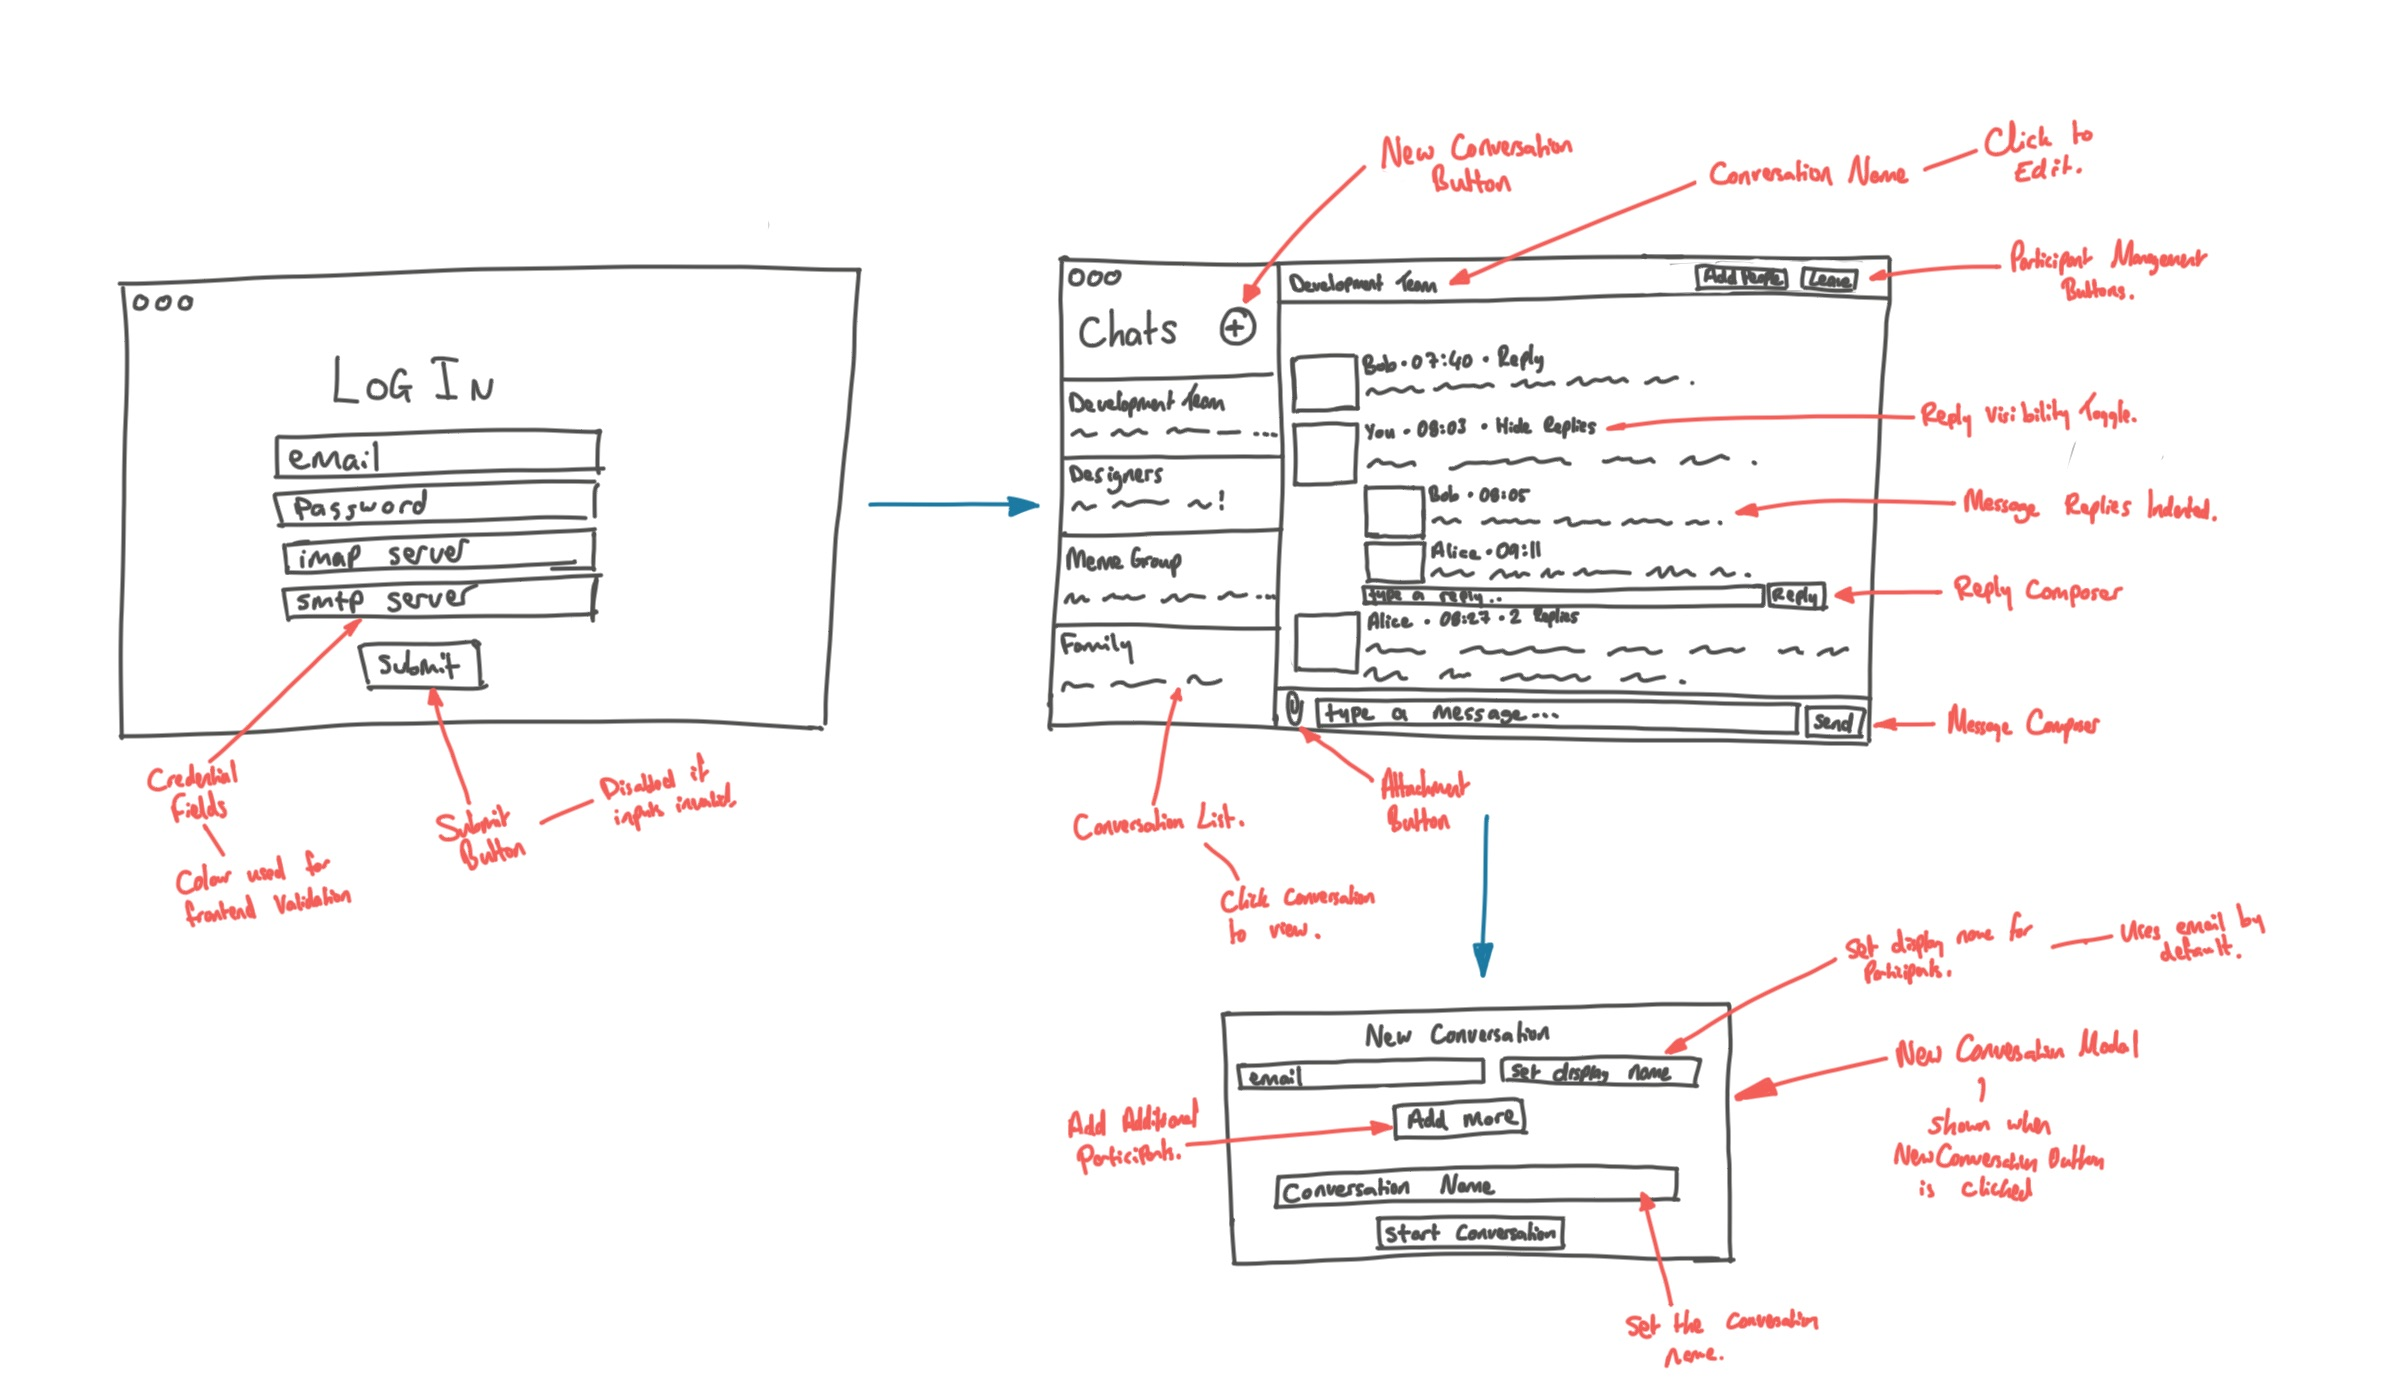
\includegraphics[width=\textwidth]{images/wireframes.jpg}
  }
  \caption{Low-fidelity wireframe showing the key user interface elements}
  \label{fig:ui-wireframes}
\end{figure}

Using these essential UI elements some low-fidelity wireframes were produced, seen in Figure \ref{fig:ui-wireframes}. The wireframes have deliberately been created at a high-level, without large amounts of detail, to allow for changes as the project progresses through the Agile development process. These wireframes will be used to support building a user interface using React, however it is noted that the specifics of the design will likely change over time as the project evolves and user feedback is gathered. The designs should, however, aid in decomposing the design into user interface components and allow for the development of a Minimum Viable Product.